\documentclass{beamer}
\usepackage[utf8]{inputenc}
\usepackage[czech]{babel}
\usepackage{graphics} 
\usepackage{bookman}
\usetheme{Madrid}
\bibliographystyle{czplain}
\providecommand{\uv}[1]{\quotedblbase #1\textquotedblleft}
 
%titulní strana
\title{Apple Inc.}
\author{Petr Jůda}
\institute{ITY - projekt 5}
\date{2016}
 
\begin{document}
\frame{\titlepage}
 
\begin{frame}
\frametitle{Historie}
\begin{itemize}
 \item Historie firmy \textsc{Apple (Computer) Inc.} sahá do roku 1976 \cite{Wikipedia:Apple}.
 \item Zakladatelé společnosti: 
 	\begin{itemize}
	\item Steve Jobs
	\item Steve Wozniak
	\item (Ronald Wayne)
	\end{itemize}
 \item Základní kapitál \$1350.
 \item Dnes jedna z nejhodnotnějších značek světa.
\end{itemize}
\end{frame}
 
\begin{frame}
\frametitle{Logo}
\begin{itemize}
 \item Logo firmy bylo ve své historii jednou změněno.
 \item Původní logo (obrázek \ref{logo1}), které vyobrazovalo sedícího Issaca Newtona pod stromem, bylo po cca 2~měsících nahrazeno světoznámým nakouslým jablkem (obrázek \ref{logo2}). \\
\begin{columns}
\column{0.5\textwidth}
\begin{figure}[h]
	\begin{center}
	\scalebox{0.30}{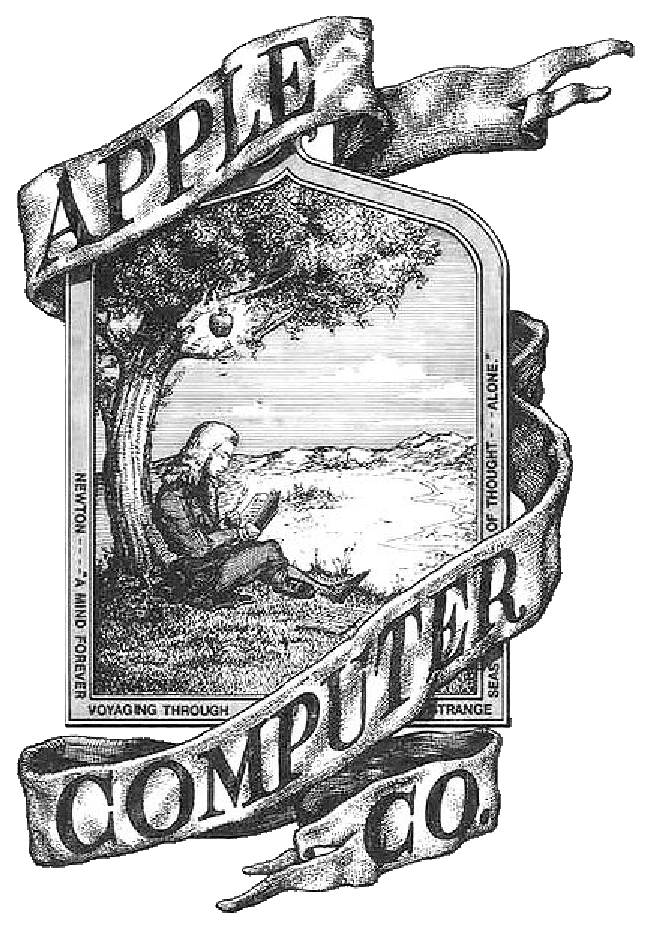
\includegraphics{logo1.eps}}
 	\caption{Původní logo Apple.}
	\label{logo1}
	\end{center}
\end{figure}

\column{0.5\textwidth}
\begin{figure}[h]
	\begin{center}
	\scalebox{1.8}{
\includegraphics{logo2.eps}}
	\caption{Původní logo Apple.}
	\label{logo2}
	\end{center}
	\end{figure}
\end{columns}
\end{itemize}
\end{frame}

\begin{frame}
\frametitle{Produktové milníky aneb čím Apple změnil svět?}
\begin{itemize}
 \item Za zmínku určitě stojí některé významné produkty \cite{MacWorld:30moments}:
 	\begin{itemize}
	\item 1984 - Mac.
	\item 1991 - PowerBook.
	\item 1993 - PDA Newton (propadák).
	\item 1998 - iMac.
	\item 2001 - iPod.
	\item 2007 - iPhone.
	\item 2010 - iPad.
	\item 2015 - Apple Watch
	\end{itemize}
\end{itemize}
\end{frame}

\begin{frame}
\frametitle{Aktuální produktová řada:}
\begin{itemize}
 \item V součastné době Apple nejvíce vydělává na těchto produktech a službách:
 	\begin{itemize}
	\item Osobní počítače iMac s OS X.11
	\item Notebooky MacBook/Pro/Air s OS X.11
	\item iPhone 6S/SE s iOS 9.3
	\item iPad Pro/Air 2 s iOS 9.3
	\item Apple Watch s WatchOS 2.1
	\item iTunes
	\item AppStore
	\item iCloud
	\item AppleTV
	\end{itemize}
 \item Velké plus si zaslouží synchronizace mezi jednotlivými zařízeními, která funguje dokonale.
\end{itemize}
\end{frame}

\begin{frame}
\frametitle{Vývojové prostředí Xcode}
\begin{itemize}
 \item Xcode je vývojové prostředí primárně pro jazyky: 
 	\begin{itemize}
	\item C/C++
	\item Obective C
	\item Swift
	\end{itemize}
 \item Vytvářet a kompilovat můžete i jiné projekty.
 \item Xcode obsahuje debbuger, integrované propojení s Gitem a veškeré simulátory potřebné pro vývoj aplikací pod OS X, iOS i WatchOS.
 \item Propojení s Apple Developer Account umožňuje nabízet své aplikace v prostředí AppStore.
\end{itemize}
\end{frame}

\begin{frame}
\frametitle{Zajímavosti:}
\begin{itemize}
 \item Steve Jobs byl po představení prvního Macintoshe z firmy vyhozen, později se do firmy vrátil jako nový ředitel.
 \item Inspirací pro název Macintosh byl název odrůdy jablek McIntosh.
 \item Bill Gates v roce 1997 investoval do Applu 150 milionů dolarů, aby jej zachránil před totálním bankrotem \cite{Tarifomat:Zajimavosti}.
 \item Kouřením u počítačů Apple zaniká nárok na záruku \cite{Tarifomat:Zajimavosti}.
\end{itemize}
\end{frame}

\begin{frame}
\frametitle{Konec}
\center
	\uv{ Stay Hungry. Stay Foolish.}\\ 
	 Steave Jobs
\end{frame}

\begin{frame}
 \frametitle{Zdroje:}
 \bibliography{odkazy}
\end{frame}
\end{document}